\documentclass[tikz,border=8pt]{standalone}
% Shared look for every TikZ diagram. Load with % Shared look for every TikZ diagram. Load with % Shared look for every TikZ diagram. Load with \input{../../tools/tikz-style.tex}
\usepackage[T1]{fontenc}
\usepackage{lmodern}
\renewcommand{\sfdefault}{lmr}  % diagrams use the same serif as the text
\usetikzlibrary{arrows.meta, positioning, shapes.geometric, calc, fit, backgrounds}
\definecolor{cblue}{HTML}{4C78A8}
\definecolor{corange}{HTML}{F58518}
\definecolor{cgreen}{HTML}{54A24B}
\definecolor{cred}{HTML}{E45756}
\definecolor{cpurple}{HTML}{B279A2}
\definecolor{cgrey}{HTML}{6B6B6B}
\tikzset{
  every picture/.style={font=\sffamily, line width=1.2pt},
  box/.style={draw=#1, fill=#1!12, rounded corners=4pt, align=center, inner sep=7pt, minimum height=1.1cm},
  box/.default=cgrey,
  arrow/.style={-{Stealth[length=3mm]}, draw=cgrey, line width=1.4pt},
  title/.style={font=\sffamily\bfseries\Large},
  note/.style={font=\sffamily\small, text=cgrey, align=center},
}
\AtBeginDocument{\hyphenpenalty=10000 \exhyphenpenalty=10000}

\usepackage[T1]{fontenc}
\usepackage{lmodern}
\renewcommand{\sfdefault}{lmr}  % diagrams use the same serif as the text
\usetikzlibrary{arrows.meta, positioning, shapes.geometric, calc, fit, backgrounds}
\definecolor{cblue}{HTML}{4C78A8}
\definecolor{corange}{HTML}{F58518}
\definecolor{cgreen}{HTML}{54A24B}
\definecolor{cred}{HTML}{E45756}
\definecolor{cpurple}{HTML}{B279A2}
\definecolor{cgrey}{HTML}{6B6B6B}
\tikzset{
  every picture/.style={font=\sffamily, line width=1.2pt},
  box/.style={draw=#1, fill=#1!12, rounded corners=4pt, align=center, inner sep=7pt, minimum height=1.1cm},
  box/.default=cgrey,
  arrow/.style={-{Stealth[length=3mm]}, draw=cgrey, line width=1.4pt},
  title/.style={font=\sffamily\bfseries\Large},
  note/.style={font=\sffamily\small, text=cgrey, align=center},
}
\AtBeginDocument{\hyphenpenalty=10000 \exhyphenpenalty=10000}

\usepackage[T1]{fontenc}
\usepackage{lmodern}
\renewcommand{\sfdefault}{lmr}  % diagrams use the same serif as the text
\usetikzlibrary{arrows.meta, positioning, shapes.geometric, calc, fit, backgrounds}
\definecolor{cblue}{HTML}{4C78A8}
\definecolor{corange}{HTML}{F58518}
\definecolor{cgreen}{HTML}{54A24B}
\definecolor{cred}{HTML}{E45756}
\definecolor{cpurple}{HTML}{B279A2}
\definecolor{cgrey}{HTML}{6B6B6B}
\tikzset{
  every picture/.style={font=\sffamily, line width=1.2pt},
  box/.style={draw=#1, fill=#1!12, rounded corners=4pt, align=center, inner sep=7pt, minimum height=1.1cm},
  box/.default=cgrey,
  arrow/.style={-{Stealth[length=3mm]}, draw=cgrey, line width=1.4pt},
  title/.style={font=\sffamily\bfseries\Large},
  note/.style={font=\sffamily\small, text=cgrey, align=center},
}
\AtBeginDocument{\hyphenpenalty=10000 \exhyphenpenalty=10000}

\begin{document}
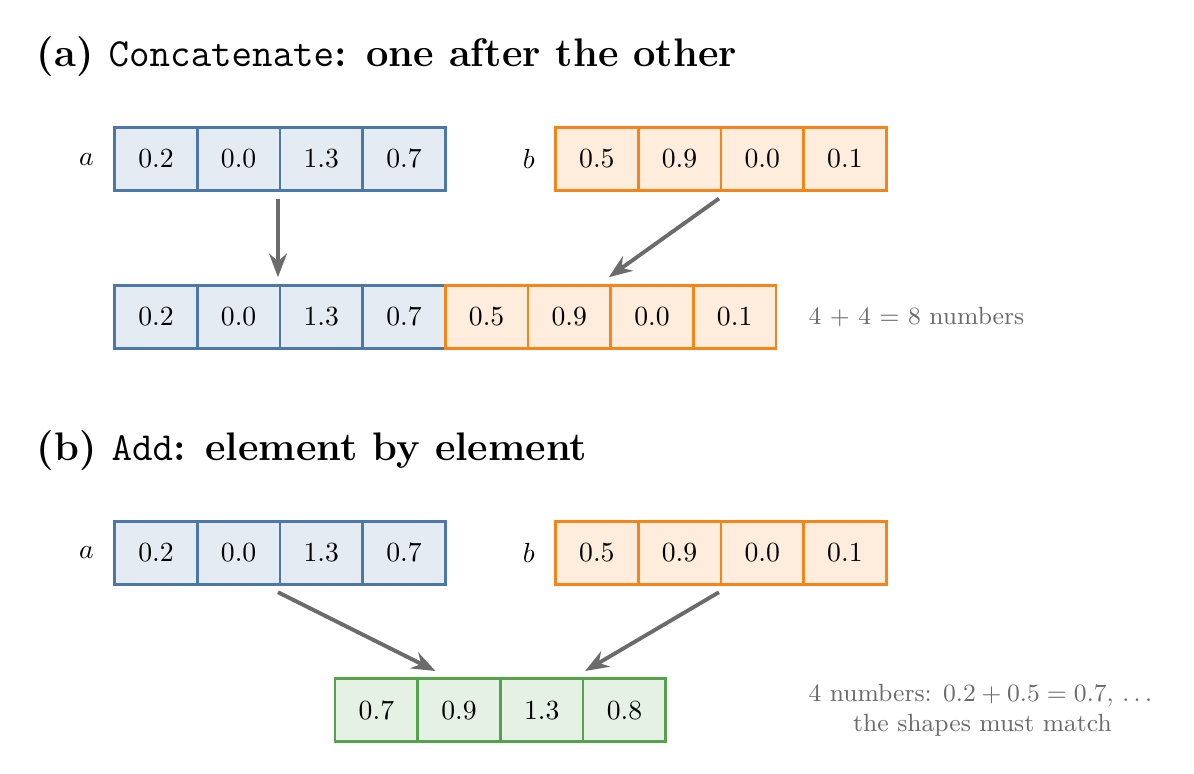
\begin{tikzpicture}[c/.style={draw=#1, fill=#1!15, minimum width=1.05cm, minimum height=0.8cm, font=\sffamily, line width=1pt}]
  \def\A{0.2,0.0,1.3,0.7} \def\B{0.5,0.9,0.0,0.1}
  % (a) Concatenate
  \node[title, anchor=west] at (-0.6, 1.3) {(a) \texttt{Concatenate}: one after the other};
  \foreach \v [count=\i] in \A {\node[c=cblue] at (\i*1.05, 0) {\v};}
  \node[anchor=east] at (0.4, 0) {$a$};
  \foreach \v [count=\i] in \B {\node[c=corange] at (\i*1.05 + 5.6, 0) {\v};}
  \node[anchor=east] at (6.0, 0) {$b$};
  \foreach \v [count=\i] in \A {\node[c=cblue] at (\i*1.05, -2.0) {\v};}
  \foreach \v [count=\i] in \B {\node[c=corange] at (\i*1.05 + 4.2, -2.0) {\v};}
  \draw[arrow] (2.6, -0.5) -- (2.6, -1.5); \draw[arrow] (8.2, -0.5) -- (6.8, -1.5);
  \node[note, anchor=west] at (9.2, -2.0) {4 + 4 = 8 numbers};
  % (b) Add
  \node[title, anchor=west] at (-0.6, -3.7) {(b) \texttt{Add}: element by element};
  \foreach \v [count=\i] in \A {\node[c=cblue] at (\i*1.05, -5.0) {\v};}
  \node[anchor=east] at (0.4, -5.0) {$a$};
  \foreach \v [count=\i] in \B {\node[c=corange] at (\i*1.05 + 5.6, -5.0) {\v};}
  \node[anchor=east] at (6.0, -5.0) {$b$};
  \foreach \v [count=\i] in {0.7,0.9,1.3,0.8} {\node[c=cgreen] at (\i*1.05 + 2.8, -7.0) {\v};}
  \draw[arrow] (2.6, -5.5) -- (4.6, -6.5); \draw[arrow] (8.2, -5.5) -- (6.5, -6.5);
  \node[note, anchor=west] at (9.2, -7.0) {4 numbers: $0.2 + 0.5 = 0.7$, \dots\\the shapes must match};
\end{tikzpicture}
\end{document}
